\documentclass{article}

\usepackage[english]{babel}
\setlength\parindent{0pt} % Removes all indentation from paragraphs
%\usepackage{times} % Uncomment to use the Times New Roman font

\usepackage{color}
	\definecolor{darkred}{rgb}{0.55, 0.0, 0.0}
	\definecolor{keywords}{RGB}{255,0,90}
	\definecolor{comments}{RGB}{0,0,113}
	\definecolor{red}{RGB}{160,0,0}
	\definecolor{green}{RGB}{0,150,0}

\usepackage{amssymb,amsmath}
\usepackage{mathtools}

\usepackage{placeins}

\usepackage{wrapfig}
\usepackage{graphicx}
\usepackage{caption}
\usepackage{subcaption}

\usepackage{hyperref}

\usepackage{listings}
\lstset{language=Python, 
        basicstyle=\ttfamily\small, 
        keywordstyle=\color{keywords},
        commentstyle=\color{comments},
        stringstyle=\color{red},
        showstringspaces=false,
        identifierstyle=\color{green},
        title=\lstname}
%------------------------------------------------------------------------------%
%------------------------------------------------------------------------------%                                   
\title{Machine Learning \\ \bf{Exercise 5: Application of the linear regression
								in tomography} } % Title
%------------------------------------------------------------------------------%                                   
% Document
%------------------------------------------------------------------------------%                                   

\begin{document}

\maketitle

\begin{center}
\begin{tabular}{l l}
Group: &  Sergej Kraft \\
       & Elias Roeger \\
       & Ekaterina Tikhoncheva \\ 
\end{tabular}
\end{center}

\tableofcontents

\section{Construction of A}

To construct matrix $A$ we adopted the idea, that sensor is places in the middle of the image $x$ and that coordinate center also lies in the middle of the image $x$.

For each image pixel $(x,y)$, where $x=-\frac{(N-1)}{2}\dots\frac{(N-1)}{2}, y=-\frac{(N-1)}{2}\dots\frac{(N-1)}{2}$ and $N$ is the size of the image, we calculated it's projection on the sensor line. The equation of the sensor line is $y=\tan(180^\circ-\alpha) x$ and the coordinates of the projection $(px,py)$ of the pixel $(x,y)$ are described by:
$$\begin{cases}
px = \frac{x+\tan(180^\circ-\alpha)y}{\tan(180^\circ-\alpha)^2+1} \\
py = \tan(180^\circ-\alpha) px
\end{cases}$$

According to the values $(px,py)$ one decides, which sensor pixel receives the corresponding ray passing through the pixel $(x,y)$. The sensor pixel, which is the closest to the projection point, is selected. The value of this sensor pixel will be increased by the intensity of the ray. The intensity of the ray is a function of the distance between image pixel and sensor pixel. We used the function $f(dist) = N - dist$.

If an ray crosses the sensor in between of two centres of the sensor pixels, than it's intensity is divided between those sensor pixel and absorbed value is calculated by the formula $\frac{intensity*(dist_{s_1}+dist_{s_2} - dist_{s_i})}{dist_{s_1}+dist_{s_2}}$, where $intensity$ is the intensity of the ray, $dist_{s_i}$ is the distance between projection $(px, py)$ and center of the sensor pixel $s_i, i=1,2$.

The listing of the function $makeA(shape, alphas)$ with $numpy$ arrays can be found below:

\begin{lstlisting}[language=Python]
#-----------------------------------------------------------------------------
def makeA_numpyArray(shape, alphas):
    assert shape[0]==shape[1], 'Expect square matrix'
    
    N = shape[0]    # NxN shape of the image
    M = len(alphas) # number of alphas
    K = int(N*np.sqrt(2))
    
    if K%2==0:
        K = K + 1   # sensor length is always a odd number
    
    sensorcenter = np.zeros((2,K), dtype = np.float32)
    A = np.zeros((M*K, N*N), dtype = np.float32)    
    
    for a in range(0,M):
        
        alpha = alphas[a]
        ralpha = np.pi*(180 - alpha)/180. # alpha in radians
                        
        for s in range(0,K):
            if alpha==-90 or alpha== 90:
                sensorcenter[0][s]= 0
                sensorcenter[1][s]= np.sign(alpha)*(K -s -1 - (K-1)/2) 
            else :                 
                sensorcenter[0][s]= np.cos(ralpha)*(K - s - 1 - (K-1)/2 ) 
                sensorcenter[1][s]= np.sin(ralpha)*(K - s - 1 - (K-1)/2 ) 
        # end for i
                
        # for each pixel calculate contribution to absorption along a rai
        for i in range(0,N*N):
                            
            # coordinates of the image pixel
            # (coordinate center is shifted to the picture center)
            x = i%N - (N-1)/float(2)
            y = i/N - (N-1)/float(2)
            
            # px,py - projection of the pixel on the sensor 
            if alpha==-90 or alpha == 90:           
                py = y
                px = 0                    
            else:
                px = (y*np.tan(ralpha)+x)/(np.tan(ralpha)*np.tan(ralpha)+1)
                py = np.tan(ralpha)*px
            # end if
            
            distToProj = np.abs(x*np.tan(ralpha)-y)/ \
                         np.sqrt(np.tan(ralpha)*np.tan(ralpha) + 1)
                         
            pixelcontribution = N-distToProj
            
            #distance between projection of (x,y) and centers of the sensorpixel
            dist =  np.zeros(K, dtype = np.float32)
            for s in range(0,K):
                dist[s] = (sensorcenter[0][s]-px)*(sensorcenter[0][s]-px)\
                        + (sensorcenter[1][s]-py)*(sensorcenter[1][s]-py)
                dist[s] = np.sqrt(dist[s])
            #end for s
            
            # find receiver sensorpixel
            ind = np.argsort(dist)

            if np.abs(dist[ind[0]]-0.5)> 0.1:
                A[a*K+ind[0]][i] += pixelcontribution
            else :
                # if ray meets sensor in between of two sensor pixels                          
                # intensity of the ray is devided between those pixels
                A[a*K+ind[0]][i] += pixelcontribution*(dist[ind[0]]/ \
                                                (dist[ind[0]]+dist[ind[1]]))
                A[a*K+ind[1]][i] += pixelcontribution*(dist[ind[1]]/ \
                                                (dist[ind[0]]+dist[ind[1]]))
            #end if                
        #end for i
    #end for alpha  
                
    return A
# end def makeA    
#-----------------------------------------------------------------------------
\end{lstlisting}


\begin{figure}[ht]
        \centering
        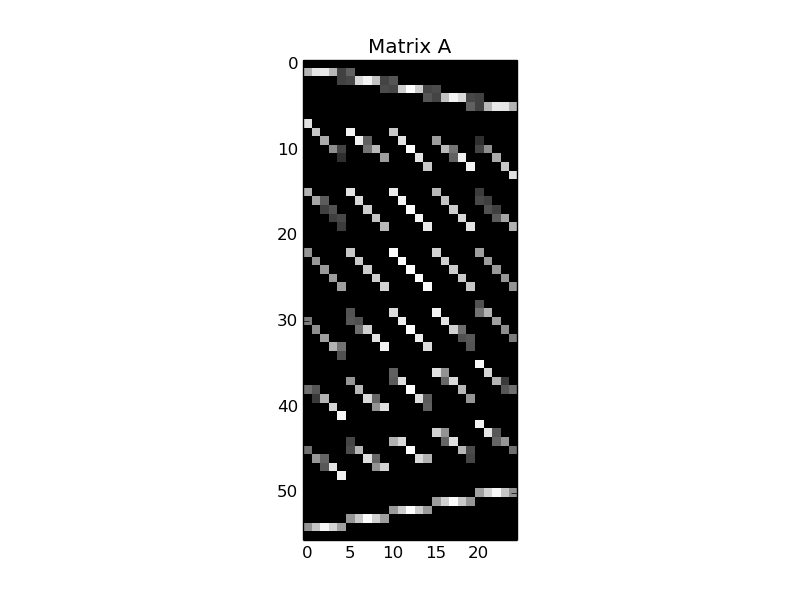
\includegraphics[width=\textwidth]{../matrixA.png}
        \caption{Matrix A for the image $5\times5$ and angles $[-77,\ -33,\ -12,\ 3,\ 21,\ 42,\ 50,\ 86]$ }
        \label{img1}
\end{figure}
\FloatBarrier

\section{Reconstruction of the image}

The results of the image reconstruction for two sets of arrays $(y,\alpha)$ are shown on the images \ref{img2} and \ref{img3}.

\begin{figure}[hb]
        \centering
        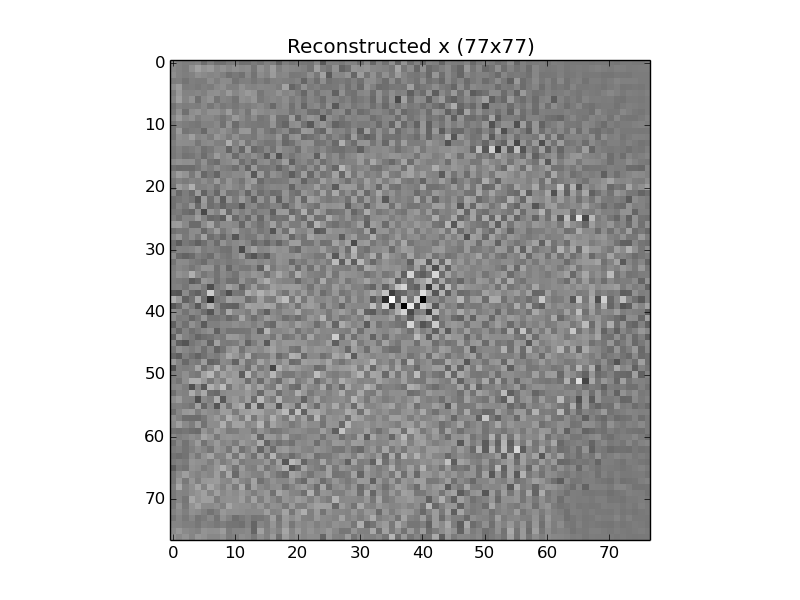
\includegraphics[width=0.3\textwidth]{../x_77.png}
        \caption{Reconstruction of the image x ($77\times77$)}
        \label{img2}
\end{figure}

\FloatBarrier

\begin{figure}[ht]
        \centering
        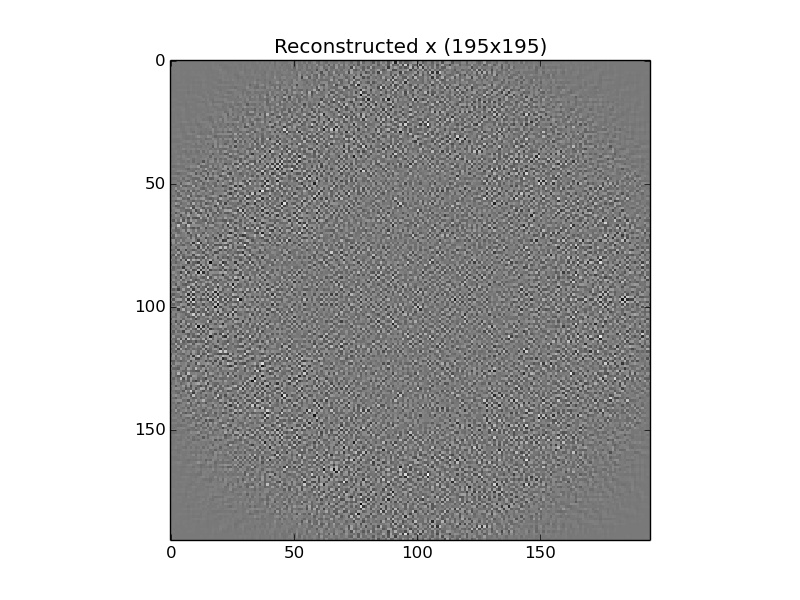
\includegraphics[width=0.3\textwidth]{../x_195.png}
        \caption{Reconstruction of the image x ($195\times195$)}
        \label{img3}
\end{figure}
\FloatBarrier

From the first image we can recognize the patient H.S., but because of the image quality we cann't state the cause of the headache by the patient.
Probably the reason for this is the calculation of the Ray intensity. We used simple line function (see section $1$).

\section{Minimization of the radiation doze}

By the image size $77\times 77$ we tried to reduce in half projection number. In this case it was not possible to recognize anything (see image \ref{img4}).

\begin{figure}[htb]
        \centering
        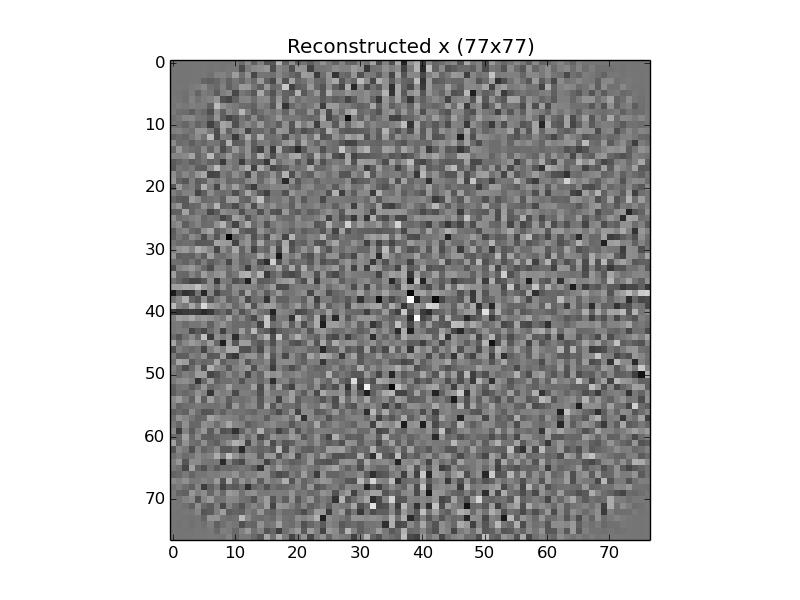
\includegraphics[width=0.3\textwidth]{../x_77r.png}
        \caption{Reconstruction of the image x ($77\times77$)}
        \label{img4}
\end{figure}
\FloatBarrier

\section{Listing $ex05.py$}
\lstinputlisting[language=Python]{../ex05.py}

\end{document}
%------------------------------------------------------------------------------%                                    
